\chapter{Contrastive Learning como Primera Solución al Colapso}
\label{cap:contrastive}

Habiendo mostrado en el capítulo anterior que $\mathcal{L}_{pos}$ actúa como un operador de contracción que degenera el espacio de representaciones, se introduce la idea de \textit{Contrastive Learning} como primera técnica para resolver el problema del colapso de $\mathcal{Z}$. Este paradigma contrarresta la dinámica contractiva mediante un término repulsivo en la función de pérdida que penaliza la proximidad entre representaciones de conceptos dispares, induciendo así una distribución más uniforme sobre $\mathcal{Z}$.


\section{Métodos Contrastivos con Margen}
\label{sec:contrastive_hadsell}

Desde la concepción original de las redes siamesas en 1993, el problema del colapso de representaciones permaneció sin solución durante más de una década, hasta la propuesta de Hadsell, Chopra y LeCun en 2006 \cite{hadsell2006dimensionality}. Este enfoque sugiere refinar el aprendizaje por pares añadiendo \textbf{pares negativos} (muestras semánticamente distintas) cuyas representaciones deben ser forzadas a separarse en el espacio latente.

\begin{definition}

Sea $(x_1, x_2)$ un par negativo, $d_W(x_1, x_2) = \| f_W(x_1) - f_W(x_2) \|_2$ la distancia euclídea en el espacio de representaciones, y $m > 0$ un hiperparámetro escalar denominado \textbf{margen}, se define la \textbf{pérdida negativa con margen} como:

\begin{equation}
\mathcal{L}_{\text{neg}}(x_{1}, x_{2}) = \max\left(0, m - d_W(x_1, x_2)\right)^2
\label{eq:L_neg}
\end{equation}

\end{definition}

Esta función penaliza a los pares negativos cuando la separación entre sus representaciones a es inferior al margen de seguridad $m$.

Dado que en el Capítulo~\ref{cap:siamesas_colapso}, hacíamos uso de la \textbf{pérdida positiva} $\mathcal{L}_{\text{pos}}$, cuya función era aproximar las representaciones de pares similares:
\begin{equation}
\mathcal{L}_{\text{pos}}(x_1, x_2) = d_W(x_1, x_2)^2
\label{eq:L_pos_cap4}
\end{equation}

Podemos ahora definir una función objetivo global asignando una variable binaria de etiqueta $Y \in \{0, 1\}$ a cada par de entradas $(x_1, x_2)$:
\begin{equation}
Y = \begin{cases}
1 & \text{si el par es positivo (semánticamente similar)} \\
0 & \text{si el par es negativo (semánticamente distinto)}
\end{cases}
\end{equation}
\vspace{2pt}

\begin{definition}[Pérdida Contrastiva con Margen]
    
La \textbf{pérdida contrastiva} poblacional se construye combinando ambas dinámicas bajo la esperanza sobre la distribución conjunta $p(x_1, x_2, Y)$:
\begin{equation}
\mathcal{L}_{\text{cont}}(W) = \frac{1}{2} \mathbb{E} \left[ Y \cdot \mathcal{L}_{\text{pos}} + (1 - Y) \cdot \mathcal{L}_{\text{neg}} \right]
\label{eq:L_cont}
\end{equation}

Su equivalente empírico sobre un conjunto de $N$ pares viene dado por:
\begin{equation}
\hat{\mathcal{L}}_{\text{cont}}(W) = \frac{1}{2N} \sum_{i=1}^{N} \left[ Y_i \mathcal{L}_{\text{pos}}^{(i)} + (1 - Y_i) \mathcal{L}_{\text{neg}}^{(i)} \right]
\label{eq:L_cont_empirica}
\end{equation}
\end{definition}

La optimización de ${\mathcal{L}}_{\text{cont}}$ induce dinámicas atractivas y repulsivas (Figura~\ref{fig:contrastive_forces}):

\begin{itemize}
    \item \textbf{Dinámica atractiva ($Y=1$): } Los pares positivos activan exclusivamente $\mathcal{L}_{\text{pos}}$, minimizando $d_W^2$ para reducir la distancia entre embeddings de muestras similares. De forma que, su gradiente actúa como una fuerza de atracción.
    
    \item \textbf{Dinámica repulsiva ($Y=0$): } Pares que negativos activan exclusivamente $\mathcal{L}_{\text{neg}}$, minimizando $\max(0, m - d_W)^2$. Cuando dos muestras distintas se encuentran a distancia inferior al margen ($d_W < m$), el término se activa y genera un gradiente que separa sus embeddings. En caso contrario $\mathcal{L}_{\text{neg}}= 0$, es decir, la red no aleja representaciones que ya son suficientemente "distintas" forzando al modelo a concentrar su capacidad en los pares negativos aún no resueltos.
\end{itemize}



\begin{figure}[H]
\centering
\begin{tikzpicture}[>=Stealth, node distance=2cm]

    % --- Fuerzas de Atracción (Positivos) ---
    \node[align=center, font=\small] (title_pos) at (-4, 2.2) {\textbf{Pares Positivos} ($Y=1$) \\ Atracción tipo Muelle};
    
    \node[circle, fill=blue!15, draw=blue, thick, minimum size=0.8cm] (p1) at (-5.4, 0) {$z_1$};
    \node[circle, fill=blue!15, draw=blue, thick, minimum size=0.8cm] (p2) at (-2.6, 0) {$z_2$};
    
    % Flechas gruesas simulando atracción
    \draw[->, ultra thick, blue] (p1.east) -- ++(0.9, 0);
    \draw[->, ultra thick, blue] (p2.west) -- ++(-0.9, 0);
    \node[blue, font=\small\bfseries] at (-4, -2.2) {Atracción: $\mathbf{F} \propto d_W$};

    % --- Fuerzas de Repulsión (Negativos, d < m) ---
    \node[align=center, font=\small] (title_neg_in) at (1, 2.2) {\textbf{Pares Negativos} ($Y=0$) \\ Repulsión activa ($d_W < m$)};
    
    \node[circle, fill=red!15, draw=red, thick, minimum size=0.8cm] (n1_in) at (1, 0) {$z_1$};
    
    % Margen
    \draw[dashed, red, thick] (n1_in) circle (1.6cm);
    \draw[->, red, densely dotted] (n1_in.center) -- ++(-1.6, 0) node[midway, above, font=\footnotesize] {$m$};
    
    \node[circle, fill=red!15, draw=red, thick, minimum size=0.8cm] (n2_in) at (2.1, 0.7) {$z_2$};
    
    % Fuerzas empujando
    \draw[->, ultra thick, red] (n1_in) -- ++(-1.0, -0.7);
    \draw[->, ultra thick, red] (n2_in) -- ++(1.0, 0.7);
    \node[red, font=\small\bfseries] at (1, -2.0) {Repulsión ($\mathbf{F} > 0$)};

    % --- Sin Fuerzas (Negativos, d >= m) ---
    \node[align=center, font=\small] (title_neg_out) at (6, 2.2) {\textbf{Pares Negativos} ($Y=0$) \\ Reposo ($d_W \ge m$)};
    
    \node[circle, fill=gray!15, draw=gray, thick, minimum size=0.8cm] (n1_out) at (6, 0) {$z_1$};
    \node[circle, fill=gray!15, draw=gray, thick, minimum size=0.8cm] (n2_out) at (8.0, 0.8) {$z_2$};
    
    % Margen
    \draw[dashed, gray, thick] (n1_out) circle (1.6cm);
    \draw[->, gray, densely dotted] (n1_out.center) -- ++(-1.6, 0) node[midway, above, font=\footnotesize] {$m$};
    
    \node[gray, font=\small\bfseries] at (6, -2.0) {Reposo ($\mathbf{F} = 0$)};
\end{tikzpicture}
\caption{Analogía física de la Pérdida Contrastiva. \textbf{Izquierda:} Las muestras similares ($Y=1$) sufren una fuerza de atracción elástica. \textbf{Centro:} Si dos muestras distintas ($Y=0$) se encuentran dentro del margen de seguridad $m$, experimentan una fuerza de repulsión que las separa. \textbf{Derecha:} Una vez superan la distancia $m$, la fuerza repulsiva se apaga y el sistema no trata de separarlas más.}
\label{fig:contrastive_forces}
\end{figure}

\section{Dinámica de Fuerzas de Atracción y Repulsión en $\mathbb{R}^d$}
\label{sec:fuerzas_latentes}

El margen $m > 0$ actua como una barrera de energía mínima que rompe la estabilidad del estado colapsado.
Supongamos que el encoder colapsa al estado constante $f_W(x) = c$. En este estado degenerado, la distancia para cualquier par es $d_W = 0$. Evaluemos la pérdida de un par negativo bajo colapso:
\begin{equation}
\mathcal{L}_{\text{neg}} = \frac{1}{2} \max(0, m - 0)^2 = \frac{1}{2} m^2 > 0
\end{equation}
Esto implica que el colapso constante es fuertemente penalizado por el término negativo. Analicemos paso a paso el gradiente de este término para un par $(x_1, x_2)$ en el caso activo, es decir, cuando $d_W < m$.

Sea $v_W = f_W(x_1) - f_W(x_2)$ el vector diferencia en el espacio de representaciones $\mathbb{R}^d$. Podemos expresar la distancia euclídea como $d_W = \|v_W\|_2$ y reescribir el factor de pérdida activo como $\frac{1}{2} (m - \|v_W\|_2)^2$. Para calcular el gradiente de la pérdida respecto a los parámetros $W$ de la red, $\nabla_W \mathcal{L}_{\text{neg}}$, aplicando la regla de la cadena:

\begin{equation}
\nabla_W \mathcal{L}_{\text{neg}} = \nabla_W \left[ \frac{1}{2} (m - \|v_W\|_2)^2 \right] = \nabla_{v} \left[\frac{1}{2} (m - \|v_W\|_2)^2 \right] \cdot \nabla_W v_W
\end{equation}


\begin{equation}
\nabla_W \mathcal{L}_{\text{neg}} = \left( \nabla_{v} \mathcal{L}_{\text{neg}} \right)^T \nabla_W v_W
\end{equation}
donde $\nabla_{v} \mathcal{L}_{\text{neg}}$ es el gradiente de la pérdida respecto al vector diferencia, y $\nabla_W v_W$ es la matriz Jacobiana de dicho vector respecto a los pesos de la red. Procederemos a calcular cada uno de estos dos componentes, del lado derecho de la ecuación, de forma independiente.

Comenzamos calculando el primer componente derivando respecto al vector $v_W$, aplicamos de nuevo la regla de la cadena sobre la norma:

\begin{equation}
\nabla_{v} \mathcal{L}_{\text{neg}} = \frac{\partial}{\partial \|v_W\|_2} \left[ \frac{1}{2} (m - \|v_W\|_2)^2 \right] \cdot \nabla_{v} \|v_W\|_2
\end{equation}

La derivada de la norma euclidea es $\nabla_{v} \|v_W\|_2 = \frac{v_W}{\|v_W\|_2} $ , por tanto:

\begin{equation}
\nabla_{v} \mathcal{L}_{\text{neg}} = - (m - \|v_W\|_2) \cdot \frac{v_W}{\|v_W\|_2}
\end{equation}

En cuanto al segundo componente, por definición $\nabla_W v_W = \nabla_W \left(f_W(x_1) - f_W(x_2) \right) $, aplicando linealidad:
\begin{equation}
\nabla_W v_W = \nabla_W f_W(x_1) - \nabla_W f_W(x_2)
\end{equation}
donde cada término $\nabla_W f_W(x)$ representa la matriz Jacobiana del \textit{encoder} de dimensiones $d \times |W|$. Sustituyendo $\nabla_{v} \mathcal{L}_{\text{neg}}$ y $\nabla_{W} v_W$ en la primera ecuación, y recordando que $d_W = \|v_W\|_2$, obtenemos la expresión para $\nabla_{W} \mathcal{L}_{\text{neg}}$:
\begin{equation}
\nabla_W \mathcal{L}_{\text{neg}} = - \underbrace{(m - d_W)}_{\text{magnitud}} \cdot \underbrace{\frac{f_W(x_1) - f_W(x_2)}{\|f_W(x_1) - f_W(x_2)\|_2}^T}_{\text{dirección}} \left( \nabla_W f_W(x_1) - \nabla_W f_W(x_2) \right)
\end{equation}

Bajo la hipótesis de colapso total, donde $f_W(x_1) = f_W(x_2)$ y la distancia se anula ($d_W = 0$), al evaluar el límite $f_W(x_1) \to f_W(x_2)$ se observa que la dirección de la fuerza repulsiva queda definida por el vector unitario:
\begin{equation}
\label{eq:u_12_vector}
\mathbf{u}_{12} = \frac{f_W(x_1) - f_W(x_2)}{\|f_W(x_1) - f_W(x_2)\|_2}
\end{equation}

Aunque el denominador tiende a cero, el vector $\mathbf{u}_{12}$ conserva norma unitaria ($\|\mathbf{u}_{12}\|_2 = 1$). Al mismo tiempo, el módulo del término repulsivo converge al valor del margen: $(m - d_W) \to m$.

Por tanto, en situación de colapso ($d_W = 0$), el gradiente de la pérdida positiva se anula ($\nabla_W \mathcal{L}_{\text{pos}} = \mathbf{0}$), mientras que el término repulsivo ($\mathcal{L}_{\text{neg}}$) mantiene un gradiente no nulo de norma proporcional a $m$. Al no anularse el gradiente total ($\nabla_W \mathcal{L} \neq \mathbf{0}$), el estado de colapso ya no constituye un punto crítico ni un atractor local; de este modo, la fuerza neta activa desplaza la optimización fuera de esta región, dispersando las representaciones en $\mathbb{R}^d$.

\section{Límites del Muestreo Negativo y Colapso Dimensional}
\label{sec:limites_negativos}

Esta formulación contrastiva de la función de pérdida introducida por Hadsell, Chopra y LeCun \cite{hadsell2006dimensionality} delega la prevención del colapso en fuerzas de repulsión generadas por las muestras negativas. Sin embargo, este enfoque basado en un margen estático $m$ se enfrenta a ciertas limitaciones cuando la dimensión crece. Como indica LeCun \cite{lecun2022path} en su manifiesto sobre los modelos basados en energía (EBM), intentar dar forma a la superficie de energía penalizando puntos discretos resulta inescalable en alta dimensión.

\subsection{Saturación del Margen y Cobertura del Espacio}

A diferencia de formulaciones probabilísticas globales, la pérdida contrastiva (Ecuación~\ref{eq:L_cont_empirica}) opera mediante una repulsión truncada localmente. Dos representaciones distintas solo experimentan un gradiente repulsivo en la dirección del vector unitario $\mathbf{u}_{1j}$ (Ecuación~\ref{eq:u_12_vector}) si su distancia euclídea es estrictamente inferior al margen $m$.

El estado de mínima energía del sistema exige que las representaciones negativas se repelan hasta alcanzar una separación mutua de al menos $m$. Para que esta dinámica evite el colapso, el espacio debe estar densamente poblado de muestras negativas; de lo contrario, existirán regiones enteras donde ninguna muestra viola el margen $m$. Estas direcciones, al estar libres de gradiente repulsivo, son susceptibles a contraerse indefinidamente por fuerzas de atracción como pasaba en el capítulo anterior. Para garantizar que el gradiente repulsivo bloquee el colapso en todas las direcciones, cualquier punto del espacio debe encontrarse a una distancia máxima $\epsilon \le m$ de al menos una muestra negativa. A continuación formalizaremos este concepto geométrico \cite{vershynin2018high}.

\begin{definition}[$\epsilon$-red y Número de recubrimiento]
Sea $(T, d)$ un espacio métrico y sea $\epsilon > 0$. Un subconjunto $\mathcal{N} \subseteq T$ se denomina \textbf{$\epsilon$-red} ($\epsilon$-net) de $T$ si cada punto en $T$ se encuentra a una distancia menor o igual a $\epsilon$ de algún punto en $\mathcal{N}$. El \textbf{número de recubrimiento} (covering number) $\mathcal{N}(T, d, \epsilon)$ se define como la cardinalidad mínima que puede tener una $\epsilon$-red de $T$.
\end{definition}

\begin{proposition}[Cota de recubrimiento para la esfera]
Si modelamos el espacio latente acotado como la hiperesfera unitaria $\mathbb{S}^{d-1} \subset \mathbb{R}^d$, el número de recubrimiento para la distancia euclídea, denotado como $\mathcal{N}(\mathbb{S}^{d-1}, \epsilon)$, está acotado por:
\begin{equation}
\left(\frac{1}{\epsilon}\right)^d \leq \mathcal{N}(\mathbb{S}^{d-1}, \epsilon) \leq \left(1 + \frac{2}{\epsilon}\right)^d
\end{equation}
\end{proposition}

\begin{proof}[Intuición geométrica por argumento volumétrico]
La demostración completa de estas cotas se basa en un argumento volumétrico detallado por Vershynin \cite{vershynin2018high}. El razonamiento intuitivo es el siguiente:
\begin{itemize}
    \item \textbf{Cota inferior $\mathbf{(1/\epsilon)^d}$}: Para cubrir el espacio unitario, la suma de los volúmenes de las $\mathcal{N}$ bolas de radio $\epsilon$ debe ser al menos igual al volumen total del espacio original. Como el volumen de cada bola escala con la potencia $d$ de su radio, se deduce que la cantidad mínima de bolas necesarias es del orden de $(1/\epsilon)^d$.
    \item \textbf{Cota superior $\mathbf{(1+2/\epsilon)^d}$}: Se demuestra mediante un razonamiento por recubrimiento (packing) en tres pasos:
    \begin{enumerate}
        \item Tomamos un conjunto máximo de puntos en la esfera unitaria que estén separados entre sí por al menos una distancia $\epsilon$. Al ser un conjunto máximo, automáticamente forma una $\epsilon$-red (si hubiera algún punto sin cubrir, podríamos añadirlo al conjunto).
        \item Rodeamos cada uno de estos centros con una pequeña bola de radio $\epsilon/2$. Como los centros distan al menos $\epsilon$, todas estas bolas pequeñas son estrictamente disjuntas (no se solapan).
        \item El espacio original tiene radio unitario ($\mathbb{S}^{d-1}$). Las bolas pequeñas pueden sobresalir, por lo que todo el conjunto encajará exactamente dentro de una esfera ligeramente dilatada de radio $1 + \epsilon/2$.
    \end{enumerate}
    Dado que las bolas pequeñas no se solapan, la suma de sus volúmenes no puede superar el volumen de la esfera dilatada. En $d$ dimensiones, el volumen es proporcional al radio elevado a $d$, por lo que planteamos la desigualdad:
    $$ \mathcal{N} \cdot (\epsilon/2)^d \leq (1 + \epsilon/2)^d $$
    Despejando $\mathcal{N}$, obtenemos directamente la cota superior $\mathcal{N} \leq \left(\frac{1 + \epsilon/2}{\epsilon/2}\right)^d = \left(1 + \frac{2}{\epsilon}\right)^d$.
\end{itemize}
Por inducción, al añadir dimensiones ortogonales, el volumen total crece exponencialmente, multiplicando la necesidad de centros por un factor proporcional a $1/\epsilon$ con cada nuevo eje ortogonal introducido (Figura~\ref{fig:epsilon_net_dimension}).
\end{proof}

Dado que el radio de cobertura efectivo está acotado superiormente por el margen ($\epsilon < m$), la cantidad de muestras negativas necesarias escala de forma exponencial con la dimensión $d$. Si el tamaño del lote de entrenamiento es insuficiente frente a este crecimiento de orden $\mathcal{O}((1/\epsilon)^d)$, la red espacial se fractura y aparecen zonas ciegas (regiones donde el gradiente repulsivo es nulo al no haber negativos cercanos).

\begin{figure}[H]
\centering
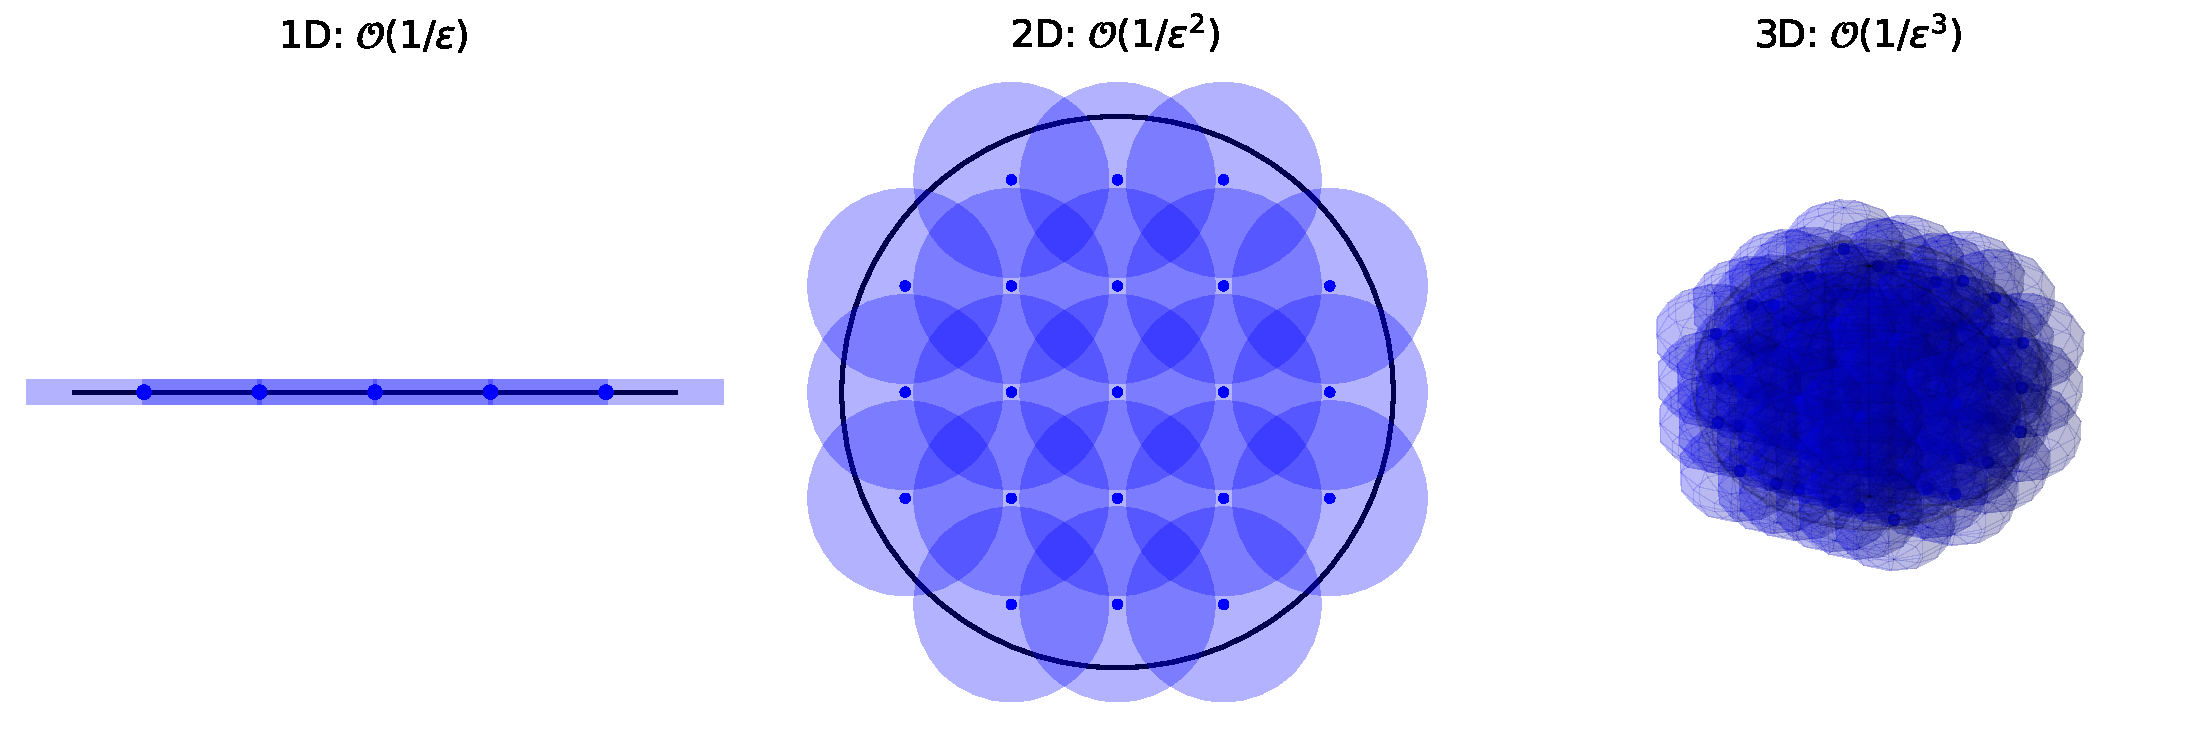
\includegraphics[width=0.95\textwidth]{epsilon_net.pdf}
\caption{Representación visual del crecimiento exponencial del número de recubrimiento $\mathcal{N}(\mathbb{S}^{d-1}, \epsilon)$. A medida que aumenta la dimensión $d$, la cantidad de muestras (centros en azul) de radio $\epsilon$ requeridas para cubrir el volumen completo sin dejar agujeros crece exponencialmente como $\mathcal{O}((1/\epsilon)^d)$.}
\label{fig:epsilon_net_dimension}
\end{figure}
